\documentclass[11pt]{article}
\usepackage[utf8]{inputenc}
\usepackage[T1]{fontenc}
\usepackage{amsmath}
\usepackage{amssymb} % Needed for \eth
\usepackage{graphicx}
\usepackage{geometry}
\usepackage{tikz}
\usepackage{pgfplots} % For plots
\usepackage{ulem}     % For underline, using normalem to avoid messing with \emph

\geometry{a4paper, margin=1in}
\usetikzlibrary{positioning, arrows.meta, shapes.geometric} % For TikZ diagrams
\pgfplotsset{compat=1.18} % Use a recent PGFPlots version

% Custom commands (optional)
\newcommand{\avg}[1]{\overline{#1}}
\newcommand{\prob}[1]{P(#1)}
\newcommand{\ProbDens}[1]{\mathcal{P}(#1)} % Using script P for density
\newcommand{\vect}[1]{\vec{#1}}
\newcommand{\dd}[1]{\mathrm{d}#1} % Differential d
\newcommand{\pderiv}[2]{\frac{\partial #1}{\partial #2}}
\newcommand{\deriv}[2]{\frac{\mathrm{d} #1}{\mathrm{d} #2}}
\newcommand{\muState}{\mu\text{-state}} % Microstate
\newcommand{\tE}{\Tilde{E}}
\newcommand{\OmegaE}{\Omega(E)}
\newcommand{\omegaE}{\omega(E)}
\newcommand{\PhiE}{\Phi(E)}
\newcommand{\deltaE}{\delta E}
\newcommand{\ethbar}{\text{\it{đ}}} % \eth symbol for inexact differential
\newcommand{\kb}{k_B} % Boltzmann constant
\newcommand{\gasR}{R} % Ideal gas constant

\title{Physics 415 - Lecture 18: Canonical Ensemble}
\date{March 3, 2025}
\author{} % Author not specified

\begin{document}

\maketitle
\thispagestyle{empty}

\section*{Summary}

\begin{itemize}
    \item Statistical description of systems:
        \begin{itemize}
            \item Classical: $\muState =$ phase space cell (Volume $(2\pi\hbar)^S$ for $S$ DOF).
            \item Quantum: $\muState =$ quantum state specified by $f$ quantum \#s $\{n_1, \dots, n_f\}$.
        \end{itemize}
    \item $\Omega(E) = \#$ accessible states with energy $E$ (or in range $(E, E+\deltaE)$).
    \item Entropy $S = \ln \Omega$.
    \item Fundamental Postulate (for isolated system in equilibrium): Probability of any accessible $\muState = 1/\Omega(E)$. (All accessible microstates are equally probable).
\end{itemize}

\section*{Return to Microscopic Statistical Approach}

Fundamental aspects have been laid out. Now learn how to calculate in various different circumstances (ensembles).

\subsection*{Microcanonical Ensemble}
In discussing the statistical approach, we have mainly dealt with an isolated/closed system.
\begin{itemize}
    \item Such a system is characterized by conserved total energy $E$ (or energy in narrow range $(E, E+\deltaE)$).
    \item Also assumed fixed particle number $N$ and fixed volume $V$ (could have other fixed external parameters, e.g., magnetization $M$, but consider only $E, N, V$ for now).
    \item In equilibrium, Prob($\muState$) $= 1/\Omega(E)$. This probability distribution is called the "microcanonical distribution".
    \item $\Omega(E) = \#$ accessible states with energy $E$.
    \item In the statistical approach, we always imagine an ensemble of $\mathcal{N} \gg 1$ similarly prepared systems.
    \item In the case of an isolated system, all members of the ensemble have the same $(E, N, V)$. An ensemble of such systems is called the "microcanonical ensemble".
\end{itemize}

\subsection*{Canonical Ensemble}

In practice, it is useful to know the statistical description of a system not at fixed energy $E$, but at fixed temperature $T$. This corresponds to a system in thermal contact with its surroundings.

Consider system A (of interest) in thermal contact with a heat reservoir A'. A' is a system much larger than A ($N' \gg N_A$, $E' \gg E_A$) that maintains system A at a constant temperature $T$.

\begin{center}
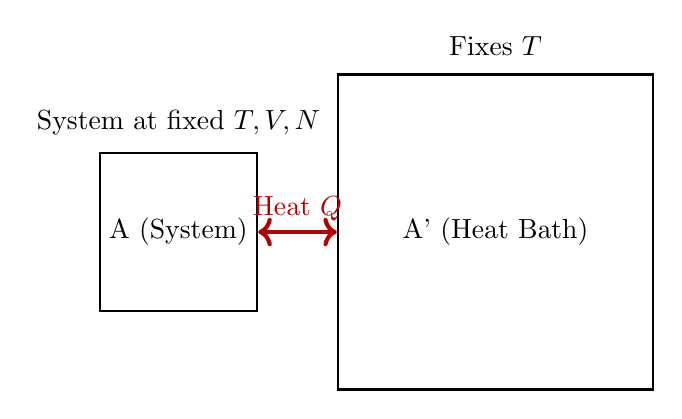
\begin{tikzpicture}
    \node (A) [draw, thick, minimum width=2cm, minimum height=2cm, label=center:A (System)] {};
    \node (Aprime) [draw, thick, minimum width=4cm, minimum height=4cm, right=1cm of A, label=center:A' (Heat Bath)] {};
    % Interface allowing heat exchange
    \draw [line width=1.5pt, red!70!black, <->] (A.east) -- (Aprime.west) node [midway, above] {Heat $Q$};
    % Labels
    \node at (A.north) [above=0.1cm] {System at fixed $T, V, N$};
    \node at (Aprime.north) [above=0.1cm] {Fixes $T$};
\end{tikzpicture}
\end{center}

The total system $A^{(0)} = A + A'$ is closed/isolated. Its total energy $E^{(0)}$ is constant.
System A is *not* closed; it can exchange energy with A'. Its energy $E_A$ fluctuates.

\textbf{Question:} What is the probability $P_r$ to find system A in any individual microstate $r$ with energy $E_r$? (Using QM description here; similar argument holds in CM).

We have studied this problem before (Lecture 7). The total energy is $E^{(0)} = E_r + E'$, where $E'$ is the energy of the reservoir A' when A is in state $r$. So $E' = E^{(0)} - E_r$.
The probability $P_r$ is proportional to the number of accessible states for the reservoir A' consistent with A being in state $r$.
\[ P_r \propto \Omega'(E') = \Omega'(E^{(0)} - E_r) \]
Now use the fact that A' is much larger than A, so $E_r \ll E^{(0)}$.
Let $S' = \ln \Omega'$ be the entropy of the reservoir A'.
\[ \Omega'(E^{(0)} - E_r) = e^{S'(E^{(0)} - E_r)} \]
Expand $S'(E^{(0)} - E_r)$ for small $E_r$:
\[ S'(E^{(0)} - E_r) \approx S'(E^{(0)}) - \left. \pderiv{S'}{E'} \right|_{E' = E^{(0)}} E_r + \dots \]
The derivative is evaluated for the reservoir at energy $E^{(0)}$, which corresponds to temperature $T$: $(\partial S' / \partial E') = 1/T$.
\[ S'(E^{(0)} - E_r) \approx S'(E^{(0)}) - \frac{E_r}{T} \]
(Here $T$ is temperature in energy units).
Substitute back into $\Omega'$:
\[ \Omega'(E^{(0)} - E_r) \approx e^{S'(E^{(0)}) - E_r/T} = e^{S'(E^{(0)})} e^{-E_r/T} = \Omega'(E^{(0)}) e^{-E_r/T} \]
Since $P_r \propto \Omega'(E^{(0)} - E_r)$ and $\Omega'(E^{(0)})$ is just a constant independent of state $r$:
\[ P_r \propto e^{-E_r/T} \]
We can write $P_r = C e^{-E_r/T}$. The normalization constant $C$ is determined by $\sum_r P_r = 1$.
\[ \sum_r C e^{-E_r/T} = C \sum_r e^{-E_r/T} = 1 \implies C^{-1} = \sum_r e^{-E_r/T} \]
This sum plays a central role in statistical physics and is called the \textbf{partition function}, denoted by $Z$:
\[ Z \equiv \sum_r e^{-E_r/T} \]
(The sum is over all possible microstates $r$ of system A).
The probability $P_r$ is then:
\[ P_r = \frac{e^{-E_r/T}}{Z} \]
This is the probability to find the system A in microstate $r$ with energy $E_r$ when it is in thermal contact with a heat reservoir at temperature $T$. This distribution is called the \textbf{Canonical Distribution} or \textbf{Gibbs Distribution}.

\textbf{Notation:} Often define $\beta \equiv 1/T$. Then $Z = \sum_r e^{-\beta E_r}$ and $P_r = e^{-\beta E_r} / Z$.

An ensemble of systems, each with the same $(N, V)$ and in thermal contact with a heat reservoir at temperature $T$, distributed according to $P_r = e^{-\beta E_r} / Z$, is called the \textbf{canonical ensemble}.

\subsection*{Averages in the Canonical Ensemble}

The average value of an observable $O$ is calculated as:
\[ \avg{O} = \sum_r P_r O_r = \frac{1}{Z} \sum_r O_r e^{-\beta E_r} \]
where $O_r$ is the value of observable $O$ in microstate $r$.

\textbf{Example:} Average energy $\avg{E}$ of system A:
\[ \avg{E} = \sum_r P_r E_r = \frac{1}{Z} \sum_r E_r e^{-\beta E_r} \]
Note that in the canonical ensemble, the energy $E$ is not fixed but fluctuates around the average value $\avg{E}$. (We will come back to the magnitude of these fluctuations).

\textbf{Classical Case:}
The canonical distribution translates to phase space. The sum over states $r$ becomes an integral over phase space, divided by the volume of a phase space cell $(2\pi\hbar)^S$.
$q=(q_1, \dots, q_S)$, $p=(p_1, \dots, p_S)$, $dq dp = dq_1 \dots dq_S dp_1 \dots dp_S$.
\begin{itemize}
    \item Partition function: $Z_{cl} = \int \frac{dq dp}{(2\pi\hbar)^S} e^{-\beta E(q,p)}$
    \item Probability density: $dP(q,p) = \frac{e^{-\beta E(q,p)}}{Z_{cl}} \frac{dq dp}{(2\pi\hbar)^S}$
    \item Average observable: $\avg{O} = \int O(q,p) dP(q,p) = \frac{1}{Z_{cl}} \int O(q,p) e^{-\beta E(q,p)} \frac{dq dp}{(2\pi\hbar)^S}$
\end{itemize}
(Note: The $(2\pi\hbar)^S$ factor arises from QM considerations. We may need to correct this later for identical particles - Gibbs paradox).

\subsection*{Probability of having Energy E}

We need to distinguish between $P_r$ (probability of being in a specific microstate $r$) and $P(E)$ (probability that the system has energy $E$, or energy in range $(E, E+\deltaE)$).
\[ P(E) = \sum_{r \text{ s.t. } E \le E_r < E+\deltaE} P_r \]
Assuming $\deltaE$ is small so $E_r \approx E$ in the sum:
\[ P(E) \approx \sum_{r \text{ s.t. } E \le E_r < E+\deltaE} \frac{e^{-\beta E_r}}{Z} \approx \frac{e^{-\beta E}}{Z} \sum_{r \text{ s.t. } E \le E_r < E+\deltaE} (1) \]
The sum $\sum'(1)$ is just the number of states in the energy range $(E, E+\deltaE)$, which is $\Omega(E) = \omega(E)\deltaE$.
\[ P(E) \approx \frac{\Omega(E) e^{-\beta E}}{Z} \]
$P(E)$ depends on the product of the rapidly increasing function $\Omega(E)$ and the rapidly decreasing function $e^{-\beta E}$ (Boltzmann factor). The result is a function $P(E)$ that is sharply peaked at some energy $\tE = \avg{E}$. The peak becomes sharper as the size of the system A (number of DOF) increases.

\begin{center}
\begin{tikzpicture}
\begin{axis}[
    xlabel=$E$, ylabel=Probability Density $P(E)$,
    xtick=\empty, ytick=\empty,
    xmin=0, xmax=10, ymin=0,
    axis lines=left,
    samples=101, smooth, domain=0.1:10
]
% Omega(E) ~ E^N (rapidly increasing)
\addplot [blue, dashed, thick] {x^5} node[pos=0.8, anchor=south west] {$\Omega(E)$};
% exp(-beta E) (rapidly decreasing)
\addplot [red, dashed, thick] {200*exp(-1.5*x)} node[pos=0.2, anchor=south east] {$e^{-\beta E}$};
% Product P(E) (peaked)
\addplot [black, very thick] {200*x^5 * exp(-1.5*x)} node[pos=0.6, anchor=west] {$P(E) \propto \Omega(E)e^{-\beta E}$};
% Peak position
\draw [gray, dotted] (axis cs:3.33, 0) -- (axis cs:3.33, 270) node[pos=1.1, above] {$\avg{E}$}; % Peak at E = N/beta = 5/1.5 = 3.33
\draw [<->] (axis cs:2.8, 50) -- (axis cs:3.8, 50) node[midway, below] {$\Delta^* E$};
\end{axis}
\end{tikzpicture}
\end{center}

\section*{Example: Maxwell Velocity Distribution}

Usually, we apply the canonical distribution when system A is macroscopic. However, it also applies if A is small, e.g., a single particle, provided it's in contact with a large reservoir A'.

Consider a classical monatomic ideal gas. Let A be a single gas particle (molecule) and A' be all the remaining $N-1$ molecules, acting as a heat reservoir at temperature $T$.
The energy of the single particle A is just its kinetic energy: $E = \frac{1}{2} m |\vec{v}|^2 = \frac{|\vec{p}|^2}{2m}$.

The canonical distribution gives the probability density in the 6D phase space $(\vec{x}, \vec{p})$ of the single particle:
\[ P(\vec{x}, \vec{p}) d^3x d^3p \propto e^{-\beta E(\vec{p})} d^3x d^3p = e^{-\beta p^2 / (2m)} d^3x d^3p \]
The probability that the particle's position is in range $(\vec{x}, \vec{x}+d^3x)$ and its momentum is in range $(\vec{p}, \vec{p}+d^3p)$.

We are often interested in the momentum distribution alone, irrespective of position. We integrate over $\vec{x}$:
\[ g(\vec{p}) d^3p = \left( \int d^3x P(\vec{x}, \vec{p}) \right) d^3p \]
Assuming $P$ is uniform in position over the volume $V$, $\int d^3x = V$.
\[ g(\vec{p}) d^3p \propto V e^{-\beta p^2 / (2m)} d^3p \]
The momentum distribution function $g(\vec{p})$ satisfies $\int g(\vec{p}) d^3p = 1$.
Let $g(\vec{p}) = C e^{-\beta p^2 / (2m)}$. Find $C$ by normalization:
\[ C \int d^3p e^{-\beta p^2 / (2m)} = 1 \]
The integral is separable: $\int d^3p (\dots) = (\int dp_x e^{-\beta p_x^2/(2m)}) (\int dp_y \dots) (\int dp_z \dots)$.
Using the Gaussian integral $\int_{-\infty}^{\infty} e^{-ay^2} dy = \sqrt{\pi/a}$:
\[ \int_{-\infty}^{\infty} dp_x e^{-\beta p_x^2/(2m)} = \sqrt{\frac{\pi}{\beta/(2m)}} = \sqrt{\frac{2\pi m}{\beta}} = \sqrt{2\pi m T} \]
So the 3D integral is $(\sqrt{2\pi m T})^3 = (2\pi m T)^{3/2}$.
\[ C (2\pi m T)^{3/2} = 1 \implies C = (2\pi m T)^{-3/2} \]
\[ g(\vec{p}) = (2\pi m T)^{-3/2} e^{-p^2 / (2mT)} \]

To get the velocity distribution $f(\vec{v})$, use $\vec{p} = m\vec{v}$, $d^3p = m^3 d^3v$.
The probability must be the same: $g(\vec{p}) d^3p = f(\vec{v}) d^3v$.
\[ f(\vec{v}) = g(m\vec{v}) m^3 = (2\pi m T)^{-3/2} e^{-(m v)^2 / (2mT)} m^3 \]
\[ f(\vec{v}) = \left( \frac{m^6}{(2\pi m T)^3} \right)^{1/2} e^{-m v^2 / (2T)} = \left( \frac{m^3}{2\pi T^3} \right)^{1/2} e^{-m v^2 / (2T)} \]
\[ f(\vec{v}) = \left( \frac{m}{2\pi T} \right)^{3/2} e^{-m v^2 / (2T)} \]
This is the \textbf{Maxwell velocity distribution}.
$f(\vec{v}) d^3v$ = probability that a particle has velocity in the range $(\vec{v}, \vec{v}+d^3v)$.
(Remember $T$ is in energy units here. If $T$ is in Kelvin, replace $T$ with $\kb T$).

\end{document}